\documentclass[12pt]{report}

\usepackage{polski}
\usepackage[utf8]{inputenc}
\usepackage[unicode]{hyperref}
%\usepackage{bchart}
\usepackage{graphicx}
\graphicspath{ { . } }

\usepackage{indentfirst}

\usepackage{url,apacite}
\bibliographystyle{apacite}


\title{Projektowanie i tworzenie stron i aplikacji webowych}
\date{06-01-2019}
\author{Kacper Karwot}

\begin{document}
	\maketitle
	\tableofcontents
	\newpage
	\chapter{Wstęp}
	\section{Czym jest web development?}
	\textbf{Web development} to wszystkie zadania, które wchodzą w skład tworzenia strony sieci web, która może być dostępna w Internecie lub intranecie. 
	Web development to szerokie pojęcie, które może obejmować zarówno tworzenie prostej, statycznej strony zawierającej tekst lub 			skomplikowaną aplikację webową, usługę e-commerce lub serwis społecznościowy. 
 Wśród osób pracujących w branży, pojęcie "web development" zazwyczaj odnosi się do nie-projektowych aspektów budowania stron: tworzenia markupu i kodowania. Bardzo często używane są systemy zarządzania treścią(CMS) aby ułatwić dokonywanie zmian i pozwolić osobą mniej zaawansowanym technicznie na pracę nad stroną.
 	\par
 		W większych organizacjach i biznesach, zespoły web developerskie mogą liczyć nawet setki osób i pracować według takich metodologii jak Agile podczas tworzenia produktu. Przy mniejszych projektach wystarczający może być jeden stały lub kontraktowy pracownik, ewentualnie pomocnicy specjalizujący się w grafice lub technicy IT. 
	\begin{center}
	Wyróżniamy trzy rodzaje specjalizacji web developerów:
	
	\begin{itemize}
	\item[--] \textbf{front-end} developer,
	\item[--] \textbf{back-end} developer,
	\item[--] \textbf{full-stack} developer
 	\end{itemize}
 	\end{center}
 	
 	\cite{wiki:1}
 	
 	\newpage
	\section{Historia web developmentu}
	
	Tim Barners-Lee wynalazł \textit{World Wide Web} w  1989, około 20 lat po pierwszym połączeniu, które dziś jest znane 
	jako Internet. Tim był inżynierem oprogramowania w CERN, gdzie dostrzegł potencjał wymiany danych naukowych przy pomocy
	milionów komputerów połączonych ze sobą za pomocą sieci.
	\newline
	W październiku 1990 sprecyzował trzy fundamentalne technologie, które do dziś są podstawą sieci
	\begin{itemize}
	\item \textbf{HTML} -(HyperText Markup Language) - pozwala formatować dokumenty oraz linkować inne dokumenty i źródła,
	\item \textbf{URI} - (Uniform Resource Identifier) - rodzaj ''adresu'' który jest unikalny dla każdego źródła w internecie,
	\item \textbf{HTTP} -(HyperText Transfer Protocol) - który możliwia pobieranie połączonych zasobów z całej sieci
	\end{itemize}
	
	W tamtym czasie Internet stał się prawdopodobnie najpotężniejszym narzędziem wymiany danych jakiego świat doświadczył. 
	\newline
	Tim Berners-Lee i inni zrozumieli, że aby sieć Web osiągnęła swój pełen potencjał, ich fundamentalne technologie muszą stać
	się światowym standardem, implementowanym w ten sam sposób na całym świecie. W ten sposób, w 1994 roku powstało
	\textbf{World Wide Web Consortium (W3c)} jako miejsce osiągnięcia konsensusu w sprawie specyfikacji i wytycznych, aby upewnić
	się, że sieć działa dla wszystkich i rozwija się w sposób odpowiedzialny.
	
	\begin{figure}[h]
	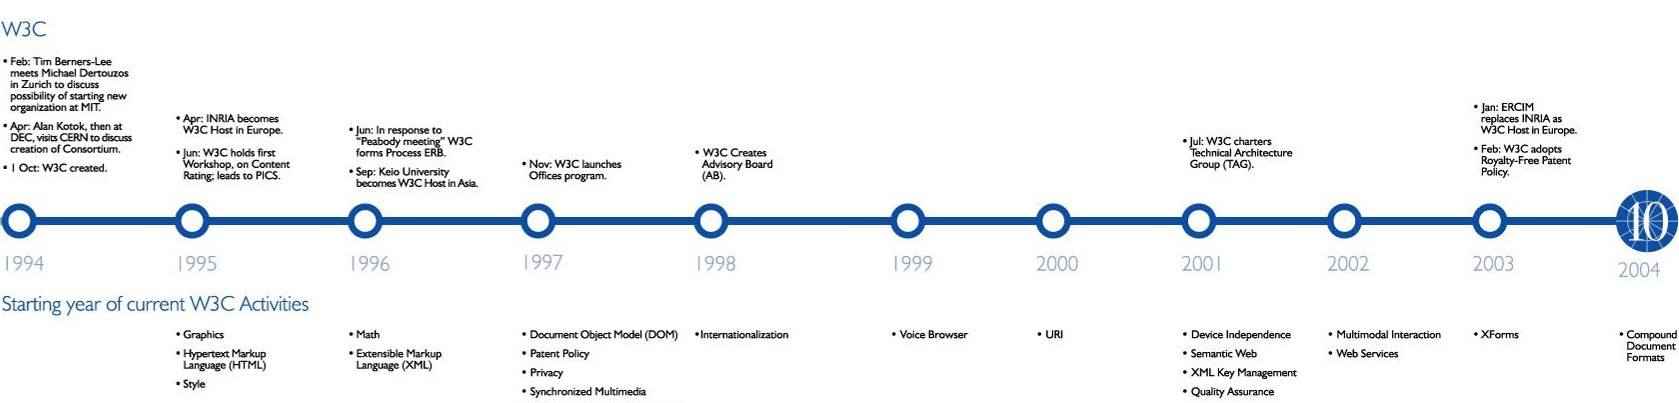
\includegraphics[width=\textwidth]{timeline.jpg}
	\caption{Oś czasu W3c}
	\end{figure}
	
	\cite{history}
	
	
%	 \begin{bchart}[max=100, unit=\%]
 %\bcbar[label={tt DP}, text=BNC,
 %color=white]{49}
 %\bcbar[text=CHILDES, color=gray!10]{35.58}
%\bcbar[text=BEE, color=gray!50]{80}
 %\bcbar[text=AMEX, color=gray!80]{100}
 %\bcxlabel{\% without CRs}
 %\end{bchart}

	\newpage
	\chapter{Kim jest web developer?}
	\section{Kto może zostać web developerem?}
	Tak naprawdę ten zawód może wykonywać każdy, kogo interesuje tworzenie stron internetowych. Jeśli planujemy w przyszłości pracować jako web developer, warto jednak zdecydować się na studia informatyczne, które będą solidną podstawą merytoryczną do dalszego rozwoju. Coraz częściej uczelnie proponują również podyplomowe kształcenie dla web developerów, na przykład Front-End Development na Politechnice Białostockiej lub Programista Aplikacji Internetowych w Wyższej Szkole Bankowej w Gdańsku. Jednak samo wykształcenie informatyczne może nie wystarczyć do zatrudnienia jako web developer. Pracodawcy zwracają dużą uwagę na doświadczenie i umiejętności. Dużym ułatwieniem w zdobyciu stanowiska związanego z kodowaniem stron www jest bogate portfolio. Dlatego warto tworzyć jak najwięcej projektów i wzbogacać swoje portfolio, którym będzie można pochwalić się w czasie spotkania rekrutacyjnego.
	\newpage
	Chcąc pracować na stanowisku web developera, trzeba koniecznie poznać również różne języki programowania i technologie. Wiedza, jaka będzie niezbędna, zależy od tego, czy projekty będą wykonywane na stanowisku front-end developer, czy back-end developer. W pierwszym przypadku chodzi o wszystko, co widać na stronie internetowej, o interfejs graficzny. Tutaj konieczne będzie poznanie HTML, CSS i JavaScript. Natomiast back-end developer zajmuje się logiką po stronie serwera i powinien znać przynajmniej jeden z takich języków programowania, jak Python, Ruby, PHP (przy okazji koniecznie trzeba zgłębić tajniki WordPressa, który z systemu dedykowanego blogom przekształcił się w jeden z najpopularniejszych obecnie CMS-ów), Java, .NET lub NodeJS. Warto także poznać najpopularniejsze frameworki, ponieważ ta wiedza może przydać się potem wielokrotnie w pracy na stanowisku web developera. W obszarze front-end trzeba zwrócić uwagę na platformy JavaScriptowe, jak AngularJS, ReactJS lub EmberJS, które wykorzystuje się do tworzenia nowoczesnych stron internetowych. Ich znajomość często nie jest wymagana, ale pomaga w awansie i jest dużym atutem przy negocjowaniu wynagrodzenia. Po stronie back-end znacznie przyspieszą development takie frameworki, jak Ruby on Rails (Ruby), Django (Python), Laravel lub Symfony2 (PHP) i Express (NodeJS). Bardzo ważne dla współczesnego web developera są również narzędzia, które znacznie ułatwiają programowanie i pozwalają zautomatyzować często powtarzane czynności (np. WebStorm).
	\cite{webd}
	
	\newpage
	\section{Czym zajmuje się web developer}
	Web developer należy do zespołu, który zajmuje się tworzeniem stron internetowych, ale jego praca skupia się na wykonaniu programistycznego zaplecza, zapewniającego serwisowi poprawne działanie. W dużym skrócie polega to na opracowaniu kodu w wybranym języku programowania i w odpowiedniej technologii. W ten sposób zostaje zapewniona odpowiednia funkcjonalność strony oraz jej właściwa budowa. Web developer projektuje i tworzy dedykowane oprogramowanie, tworzy szablony na podstawie projektów graficznych, zajmuje się opracowaniem interfejsu użytkownika, ale także przygotowuje dokumentację techniczną dla użytkownika oraz zajmuje się diagnostyką błędów w działaniu strony internetowej.
	Na co dzień web developer współpracuje z web designerem, który zajmuje się stroną graficzną strony. Czasami również ta współpraca rozszerzana jest na copywritera, dostarczającego content do serwisu oraz na administratora witryny. Praca wykonywana jest oczywiście za pomocą komputera, a kodowanie strony odbywa się zgodnie z wytycznymi zleceniodawcy. Zarobki zależą od doświadczenia, stażu oraz od zajmowanego stanowiska (Junior, Senior). W przypadku Juniora, wynagrodzenie miesięczne zwykle nie przekracza 4000 zł, natomiast zarobki Seniorów rozpoczynają się od sumy 6000 zł.
	\par
	Liczba stron internetowych nieustannie rośnie, co sprawia, że również web developerzy mają coraz więcej pracy. Muszą jednak ciągle trzymać rękę na pulsie, żeby nadążać za najnowszymi trendami w tworzeniu serwisów www, a to wymaga także nieustannego poszerzania umiejętności.
	\cite{webd}
	

	\listoffigures
	\bibliography{b.bib}

\end{document}